\documentclass{../../td}{subfiles}
\usepackage{../../raccourcis}
\begin{document}

\subsection*{Exercice I}

On considère le système 
\[
  \begin{cases}
\dot{x_1} & = x_1 +x_2\\
\dot{x_2} & = x_2^2 + u\\
y & = x_1
\end{cases}
\text{ donc } f(x) = \vect{x_1+x_2\\x_2^2}, g(x) = \vect{0 \\ 1} \et h(x) = x_1 \]

\begin{enumerate}
\item On peut balancer $u=-x_2^2 + v$ comme des bâtards mais on va suivre le cours :

\begin{enumerate}
\item Trouver le degré relatif
\begin{align*}
z_1 & = y = x_1 \\
z_2 & = \dot{y} = \dot{x_1} = x_1 + x_2, \quad r>1\\
z_3 & = \dot{z_2} = \dot{x_1} + \dot{x_2} = x_1 + x_2 + x_2^2 + u, \quad r=2
\end{align*}

\item
\[
  \begin{cases}
\dot{z_1} = z_2\\
\dot{z_2} = v
\end{cases}
\quad \text{ modèle linéaire avec } \vect{z_1 \\ z_2} = \vect{x_1 \\ x_1 + x_2} \]

\begin{align*}
u & = v - x_1 - x_2 - x_2^2 \\
& = v - z_2 - ( z_2 - z_1 )^2
\end{align*}
\end{enumerate}
\begin{figure}[ht]
  \centering
  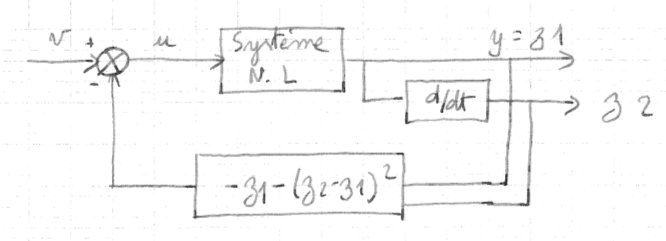
\includegraphics[width=0.9\textwidth]{1}
  \caption{ }
  \label{fig:label}
\end{figure}

%\img{0.5}{1}

\newpage
\item \[
    \begin{cases}
\dot{z_1} & = z_2 \\ \dot{z_2} & = \ddot{y} = v = \ddot{y_r} + a_1(\dot{y_r}-\dot{y})+a_2(y_r-y)
\end{cases}
\]

Équation caractéristique de la dynamique 
\[ x^2 + a_1 x + a_2 = 0 \]

%\img{0.5}{2}

\item On considère maintenant le système suivant:
\[\left\{\begin{matrix}
\dot{x_1} = x_2\\
\dot{x_2} = x_1x_2+u\\
y = x_1
\end{matrix} \right. \]

Cherchons dans un premier temps uen commande linéarisante.
\begin{align*}
z_1 = y &= x_1 = h(x)\\
z_2 = \dot{y} &= \frac{\partial h}{\partial x} \dot{x}\\
&= \begin{pmatrix}1 &0\end{pmatrix} \begin{pmatrix} x_2 \\ x_1x_2 + u\end{pmatrix}\\
&= x_2\\
\ddot{y} &= \frac{\partial \dot{y}}{\partial x} \dot{x}\\
&= \begin{pmatrix} 0 & 1\end{pmatrix} \begin{pmatrix}x_2 \\x_1x_2+u\end{pmatrix}\\
&= x_1x_2 + u = v
\end{align*}

Ainsi, $r=2$ et le modèle linéaire correspond à:
\[ \begin{pmatrix}z_1\\z_2\end{pmatrix} = \begin{pmatrix}
x_1 \\ x_2\end{pmatrix} \text{	et, } u = -x_1x_2 + v\]

Pour imposer une consigne on a alors:
\begin{align*}
\ddot{\epsilon} + a_1 \dot{\epsilon} + a_0 \epsilon = 0\\
\epsilon &= y_c - y\\
&= y_c - z_1\\
\dot{\epsilon} &= \dot{y_c} - z_2\\
\ddot{\epsilon} &= \ddot{y_c} - \dot{z_2}
\intertext{Comme $\dot{z_2} = v$ alors,}
& \ddot{y_c} - \dot{z_2} + a_1 (\dot{y_c} - z_2) + a_0 ( y_c - z_1) = 0\\
 \Rightarrow& v = \ddot{y_c} + a_1(\dot{y_c} - z_2) + a_0 ( y_c - z_1)
\end{align*}
\end{enumerate}

\subsection*{Exercice 2:}

On considère le système suivant:
\[\left\{\begin{matrix}
\dot{x_1} = x_1x_3\\
\dot{x_2} = x_1+x_2u\\
\dot{x_3} = 1 + x_3 u
\end{matrix} \right. \]

Examinons la commandabilité de ce système. Pour cela, on rappelle qu'il faut l'écrire sous la forme : 
\[\dot{x} = f(x) + g(x) u\]
On a donc m=2 et,
\begin{align*}
&f(x) = \begin{pmatrix} x_1x_2 \\ x_1 \\1\end{pmatrix}  &J_f = \begin{pmatrix}x_3 & 0 & x_1 \\ 1& 0 & 0 \\ 0 & 0 & 0\end{pmatrix}\\
&g(x) = \begin{pmatrix} 0\\ x_2 \\x_3 \end{pmatrix} &J_g = \begin{pmatrix}
0 &0&0 \\ 0&1&0 \\ 0& 0&1\end{pmatrix}
\intertext{On calcul ensuite :}
ad_fg &= [f,g] = \begin{pmatrix}-x_1x_3 \\x_1 \\ 1\end{pmatrix}\\
\text{donc, } J_{ad_fg} &= \begin{pmatrix}-x_3 & 0 & -x_1 \\ 1 & 0& 0 \\0 & 0& 0\end{pmatrix}\\
\text{reste à calculer, } ad_f^2g &= [f, ad_fg] = J_{ad_f g} - J_f ad_fg  = \begin{pmatrix}
-2 x_1 \\ 2x_1 x_3\\ 0
\end{pmatrix}
\end{align*}

Ainsi, on a $E = \{g, ad_fg, ad_f^2g\}$. Or pour $x=0$ le dernier vecteur est nul donc la dimension de E est inférieur à 3. Cela implique que le système n'est pas commandable.


\subsection*{Exercice 3:}
On considère ici le système suivant:
\[\left\{\begin{matrix}
\dot{x_1} = x_2 + u\\
\dot{x_2} = x_1^2 + x_2\\
\dot{x_3} = x_3 + u \\
y = x_1
\end{matrix} \right. \]
Déterminons la dynamique est zéros, c'est à dire que l'on va choisir $u$ de sorte à maintenir la sortie à zéro ainsi que ses dérivées successives.
Ainsi, on impose $y=0$ :
\begin{align*}
y = 0 &\Rightarrow x_1 = 0\\
&\Rightarrow \dot{x_1} = 0\\
&\Rightarrow x_2 + u = 0\\
&\Rightarrow u = -x_2\\
\text{on a aussi avec $x_1 = 0$, } &\dot{x_2} = x_2\\ 
\text{et aussi, } \dot{x_3} = x_3 - x_2
\end{align*}
On a donc la dynamique du système donnée par les valeurs propres de $ A = \begin{pmatrix}1 & 0 \\ 1 & 1\end{pmatrix}$. Les valeurs propres étant $\pm 1$, la dynamique des zéros est instable (CF début du cours de 424).


\end{document}
